\section{The objective chooses the geometry}
\label{sec:costs-zermelo}

There is no unique optimal trajectory before a functional is declared.  The
main choices are
\begin{align}
 J_T&=t_{\mathrm f},
 &J_E&=\int_0^{t_{\mathrm f}}P_{\mathrm{loss}}(\vect i,\vect u)\,\mathrm dt,
 \tag{27.1}\\
 J_u&=\int_0^{t_{\mathrm f}}\vect u^{\mathsf T}\matr W_u\vect u\,\mathrm dt,
 &J_\lambda&=\int_0^{t_{\mathrm f}}(1+\lambda P_{\mathrm{loss}})\,\mathrm dt.
 \tag{27.2}
\end{align}
Peak winding temperature additionally requires a thermal state; current slew
or torque slew can be added for acoustic and mechanical smoothness.  Minimum
time uses the boundary of the local speed body.  Minimum control energy uses a
quadratic integral and leads to a Gramian.  Minimum copper energy prices the
state itself and is closer to a finite-horizon LQR boundary-value problem.
These geometries are related, not interchangeable.

\subsection{Well-posedness audit}

\begin{table}[tb]
\centering
\caption{What prevents each dynamic objective from degenerating.}
\label{tab:dynamic-wellposed}
\begin{tabularx}{\linewidth}{@{}lXXX@{}}
\toprule
Objective & Required declaration & Compactness mechanism & Typical caveat\\
\midrule
Minimum time & bounded input, reachable target & compact \(\mathcal U\), closed state constraints & minimizer may be nonunique\\
State-loss energy & fixed time or bounded input and terminal condition & finite horizon and bounded trajectories & free time can approach an infimum without attaining it\\
Control energy & fixed positive horizon & coercive \(\matr W_u\), controllability & no amplitude guarantee\\
Time plus loss & bounded input, positive running cost & compact controls and cost \(\geq1\) & weight selects one Pareto support point\\
Thermal peak & thermal dynamics and initial temperature & bounded power and finite horizon & depends on unmeasured thermal state\\
\bottomrule
\end{tabularx}
\end{table}

In particular, minimizing \(\int\vect i^{\mathsf T}\matr R\vect i\,dt\)
without a voltage or derivative bound permits arbitrarily fast endpoint jumps
in the mathematical model.  Conversely, allowing free terminal time while
penalizing only control energy can drive the input toward zero and the time
toward infinity.  Physical voltage, current, temperature, and time bounds are
not implementation details; they create the compact feasible set on which an
optimum can exist.

\subsection{Exact Zermelo reduction}

Dynamic whitening in (26.6) produces
\[
 \dot{\vect z}_d=\vect W(\vect z_d)+\vect v,
 \qquad \|\vect v\|_2\leq1.
 \tag{27.3}
\]
This is mathematically the Zermelo navigation problem when the whitened
control body is a Euclidean ball.  For minimum time, full authority is used
almost everywhere unless a state or path constraint prevents it.  If
\(\|\vect W\|_2<1\), every local direction remains attainable.  The time
required for a tangent displacement \(\vect y\) is the positive solution of
\(\|\vect y/F-\vect W\|_2=1\):
\[
 \boxed{
 F(\vect z,\vect y)=
 \frac{\sqrt{(\vect W^{\mathsf T}\vect y)^2
 +(1-\|\vect W\|^2)\|\vect y\|^2}
 -\vect W^{\mathsf T}\vect y}
 {1-\|\vect W\|^2}.}
 \tag{27.4}
\]
This is a Randers-type Finsler metric \parencite{bao2004}.  It is positively
homogeneous in \(\vect y\) but generally nonreversible:
\(F(\vect z,\vect y)\neq F(\vect z,-\vect y)\).  The RL asymmetry of
Figure~\ref{fig:dynamic-primer}(a) is its one-dimensional shadow.

\begin{figure}[tb]
\centering
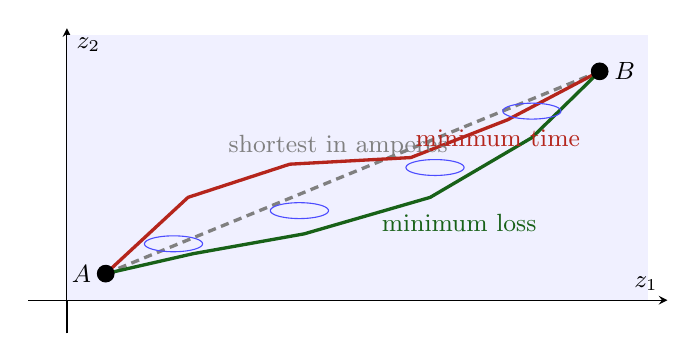
\begin{tikzpicture}[font=\small]
 \begin{axis}[width=.8\linewidth,height=.45\linewidth,axis lines=middle,
  xmin=-.4,xmax=6.2,ymin=-.5,ymax=4.1,ticks=none,xlabel={$z_1$},ylabel={$z_2$},clip=false]
  \fill[blue!6] (axis cs:0,0) rectangle (axis cs:6,4);
  \addplot[gray,densely dashed,very thick] coordinates {(.4,.4)(5.5,3.45)};
  \addplot[BrickRed,very thick] coordinates {(.4,.4)(1.25,1.55)(2.3,2.05)(3.55,2.15)(4.55,2.72)(5.5,3.45)};
  \addplot[ForestGreen!70!black,very thick] coordinates {(.4,.4)(1.3,.7)(2.45,1.0)(3.75,1.55)(4.8,2.45)(5.5,3.45)};
  \addplot[only marks,mark=*,mark size=3pt,black] coordinates {(.4,.4)(5.5,3.45)};
  \node[anchor=east] at (axis cs:.35,.4) {$A$};
  \node[anchor=west] at (axis cs:5.55,3.45) {$B$};
  \node[gray,anchor=south] at (axis cs:2.8,2.0) {shortest in amperes};
  \node[BrickRed,anchor=south west] at (axis cs:3.5,2.17) {minimum time};
  \node[ForestGreen!70!black,anchor=north west] at (axis cs:3.15,1.45) {minimum loss};
  \addplot[blue!70,thin,domain=0:360,samples=50] ({1.1+.30*cos(x)},{.85+.12*sin(x)});
  \addplot[blue!70,thin,domain=0:360,samples=50] ({2.4+.30*cos(x)},{1.35+.12*sin(x)});
  \addplot[blue!70,thin,domain=0:360,samples=50] ({3.8+.30*cos(x)},{2.00+.12*sin(x)});
  \addplot[blue!70,thin,domain=0:360,samples=50] ({4.8+.30*cos(x)},{2.85+.12*sin(x)});
 \end{axis}
\end{tikzpicture}
\caption{Core dynamic message.  Euclidean current length, minimum travel time,
and minimum transient loss select different curves.  The small local speed
bodies show the physical ruler used by the time-optimal path.}
\label{fig:geodesic-core}
\end{figure}


The statement ``minimum-time transition equals a geodesic'' is exact only
under these hypotheses: the chosen cost is time, the controlled velocity body
defines the unit ball, the drift is weak enough that the origin lies inside
the translated body, and path constraints are absent or handled as boundary
arcs.  A geodesic is then simply a locally shortest curve under the physically
induced travel-time density \(F\).

\subsection{When Randers is the wrong model}

The exact inverter hexagon crossed with an independent field-voltage interval
is not an ellipsoid.  Its gauge
\[
 \mu_{\mathcal U}(\vect u)=\inf\{\alpha>0:\vect u\in\alpha\mathcal U\}
 \tag{27.5}
\]
induces a polyhedral Minkowski norm after the linear input map.  Adding drift
still gives a Finsler travel-time density if every required tangent direction
intersects the translated velocity body, but not a Randers metric.  Corners
correspond to switching between converter facets.  An inscribed ellipsoid is
safe and smooth but conservative; a circumscribed ellipsoid is optimistic and
requires subsequent exact-converter verification.  No geometry is adopted
merely because its equations are elegant.

